Damit der Akku fachgerecht geladen wird, braucht es eine Ladeelektronik, die den LiPo-Akku nach dem CCCV-Verfahren (constant current, constant voltage) lädt. Es gab zwei Möglichkeiten, diese aufzubauen. Die eine Möglichkeit wäre ein teures IC gewesen, welches auf dem Markt verfügbar ist. Die andere Möglichkeit ist eine günstige Buck-Converter Schaltung, mit der man nach dem oberen Verfahren laden kann. Ein solcher Buck-Converter ist in diesem Produkt eingesetzt.

\begin{figure} [H]
	\centering
	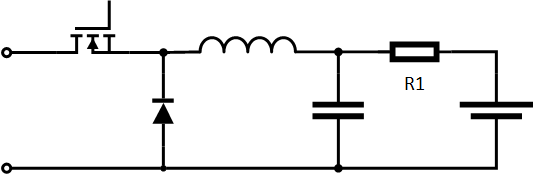
\includegraphics[width=0.6\linewidth]{images/Buck_Converter}
	\caption{Buck-Converter}
	\label{fig:Buck_Converter}
\end{figure}

Das Schema des Buck-Converters in Abbildung \ref{fig:Buck_Converter} zeigt, dass dieser einfach als auch schnell aufgebaut ist. Der Widerstand ist ein Shunt-Widerstand, an dem der Strom gemessen wird. Anhand dieses Stromes wird der PWM, welcher über einen High-Side-Treiber am MOSFET anliegt, durch den Mikrocontroller geregelt. Die Taktfrequenz des Clocks liegt bei 31.3kHz und ist mit der Formel \eqref{eqn:Taktfrequenz} aus dem Datenblatt des ATmega berechnet \cite{DatenblattATMEGA}.

\begin{equation}
f_{ PWM }=\frac { { f }_{ \mu C } }{ N\cdot256 } 
\label{eqn:Taktfrequenz}
\end{equation}

Mit dieser Taktfrequenz kann man nun die Grösse der Spule definieren. Dies wird mit folgender Formel \eqref{eqn:Spule} berechnet.

\begin{equation}
L=\frac { RF\cdot\left( { V }_{ IN }-{ V }_{ OUT } \right) \cdot\frac { { V }_{ OUT } }{ { V }_{ IN } }  }{ { f }_{ s }\cdot{ I }_{ OUT } }  
\label{eqn:Spule}
\end{equation}

Berechnet wurde eine Spule von rund 120$\mu$H. Eingesetzt ist eine Coilcraft-Spule mit dem Wert von 100$\mu$H. Da die Batterie wie ein grosser geladener Kondensator wirkt, sind keine all zu grossen Ripple am Ausgang des Buck-Converter zu erwarten.

\subsection*{Selbsterhaltung}
Wenn der LiPo-Akku voll geladen ist oder die Fahrt für mehr als 20min unterbrochen wird, sollte der Mikrocontroller sich selbstständig herunterfahren und die gesamte Stromversorgung möglichst keinen Strom brauchen. Dafür wurde eine Selbsterhaltungsschaltung entwickelt (Abbildung \ref{fig:Selbsterhaltung}). Sobald beim Mikrocontroller einer von beiden Zustände (langer Stillstand oder voll geladen) eintrifft, wird der N-Kanal-MOSFET ausgeschaltet. Somit wird die Speisung auf dem gesamten Print unterbrochen. Dadurch wird die Batterie bei einer längeren Lagerung vor dem Zerstören geschützt.

\begin{figure} [H]
	\centering
	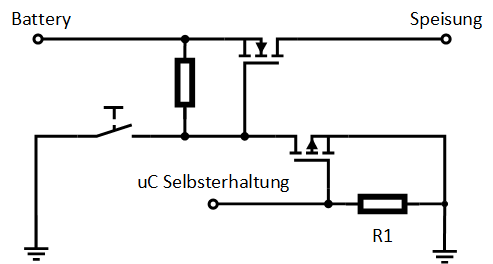
\includegraphics[width=0.6\linewidth]{images/Selbsterhaltung}
	\caption{Selbsterhaltung}
	\label{fig:Selbsterhaltung}
\end{figure}




